\documentclass[notes=show]{beamer}

\usepackage{comment}
\usepackage{default}
\usepackage[utf8]{inputenc}
\usepackage{listings}

\definecolor{OliveGreen}{cmyk}{0.64,0,0.95,0.40}
\definecolor{Gray}{gray}{0.5}

\lstset{
    language=C,
    basicstyle=\ttfamily\scriptsize,
    keywordstyle=\color{OliveGreen},
    commentstyle=\color{Gray},
    captionpos=b,
    breaklines=true,
    breakatwhitespace=false,
    showspaces=false,
    showtabs=false,
    numbers=left,
}

\begin{document}

\begin{frame}
\frametitle{Periodic Counting Network}
\begin{itemize}
\item A parallel way of counting.
\item Replaces one bottleneck (the counter) with multiple bottlenecks.
\item Maximum throughput when the number of tokens is roughly equal to the number of 
 	  balancers in the network.
\end{itemize}
\end{frame}
\note{A note} % TODO

\begin{frame}
\frametitle{Periodic Counting Network}
\begin{itemize}
\item A periodic counting network consists of a sequence of identical subnetworks.
\item Principle: Given a a number of inputs $x_i$ and outputs $y_i$ and a network width $w$,
      transform an unpredictable sequence of inputs ($x_3, x_2, x_2, x_0, x_1$) into a sequential
      output sequence ($y_0, y_1, y_2, y_3, y_0$).
\item Each thread can tell its result without consulting other counters.
\end{itemize}
\end{frame}

\begin{frame}
\frametitle{Experience}
\begin{itemize}
\item Difficult to integrate into my usual project setup (git, automated
      hand-in and unit tests).
\item Template programming requires headers-only or explicitly instantiating all
      required template instances before use.
\item As always, saturn makes life difficult by being extremely outdated,
      missing CMake files, and installing components in odd locations.
\item Algorithm in the book assumes that the network width is a power of two.
\item Not much contact with pheet.
\end{itemize}
\end{frame}

\begin{frame}[fragile]
\frametitle{Code}
\framesubtitle{incr()}
\begin{lstlisting}
template <class Pheet, typename T>
void
PeriodicCountingNetwork<Pheet, T>::incr()
{
    const int id = Pheet::get_place_id();
    out[periodic->traverse(id)].fetch_add(pcn_width, std::memory_order_relaxed);
}
\end{lstlisting}
\end{frame}

\begin{frame}[fragile]
\frametitle{Code}
\framesubtitle{get\_sum()}
\begin{lstlisting}
int
Block::traverse(const int input)
{
    const int wire = layer.traverse(input);

    if (width <= 2) {
        return wire;
    }

    if (wire < width / 2) {
        return north->traverse(wire);
    } else {
        return width / 2 + south->traverse(wire - (width / 2));
    }
}
\end{lstlisting}
\end{frame}

\begin{frame}
\frametitle{Results - Intel i5 760 Quad @ 2.80 GHz}

\begin{itemize}
\item Compiled with g++-4.8, \lstinline|-std=gnu++11 -O3|
\item 4 inputs and outputs
\end{itemize}

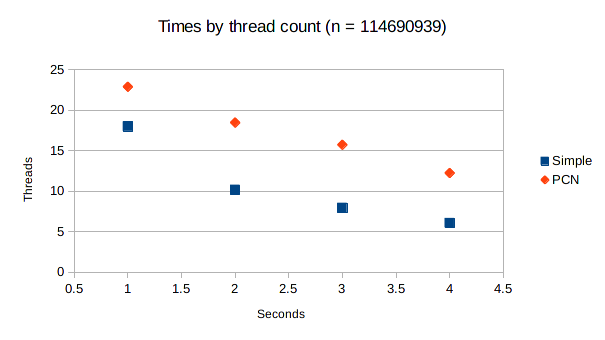
\includegraphics[width=\textwidth]{core_i5}
\end{frame}
\note{Sequential vs relaxed consistency:  virtually no difference; Simple scaled well}


\begin{frame}
\frametitle{Results - Saturn}
\begin{itemize}
\item Compiled with g++-4.7, \lstinline|-std=gnu++11 -O3|
\item 48 inputs and outputs
\end{itemize}

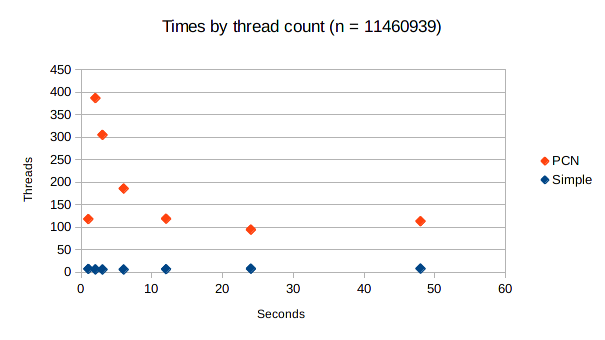
\includegraphics[width=\textwidth]{saturn}
\end{frame}
\note{Simple did not scale at all, times stayed constant.}


\begin{comment}
Reasons:
* Counting networks unsuited for this task (we don't return count after inc, thus
losing all advantages)
* Many! more instructions instead of a single fetch_and_increment
* No thread locality
* Valgrind shows nothing interesting
\end{comment}

\end{document}
